\documentclass[mathNotesPreamble]{subfiles}
\begin{document}
%\relscale{1.4} %TODO
\section{13.5: Lines and Planes in Space}\mbox{}\\[-2\baselineskip]

  \textbf{Equation of a Line:}\\
  Recall the equation of a line in $\bbr^2$:

  \noindent
  \begin{minipage}{0.5\linewidth}
    \[y=mx+b\]
  \end{minipage}%
  \begin{minipage}{0.5\linewidth}
    \begin{center}
      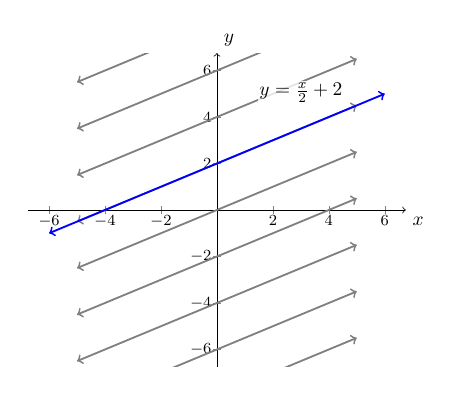
\begin{tikzpicture}[scale=0.7]
        \begin{axis}[
          axis lines=center,
          axis line style={black,->},
          xmin=-6, xmax=6,
          ymin=-6, ymax=6,
          enlargelimits={abs=0.75},
          ticklabel style={font=\footnotesize,inner sep=0.5pt,fill=white,opacity=1.0, text opacity=1},
          xlabel=$x$, xlabel style={at={(ticklabel* cs:1)},anchor=north west},
          ylabel=$y$, ylabel style={at={(ticklabel* cs:1)},anchor=south west},
          every axis plot/.append style={line width=0.95pt, color=blue, samples=100}
          ]
          \foreach \b in {-8,-6,...,8}
            {
            \addplot[<->, gray] expression[domain=-5:5]{0.5*x+\b};
            }
          \addplot[<->] expression[domain=-6:6] {0.5*x+2} 
            node[black, pos=0.75, above, yshift=12.5pt, fill=white, opacity=0.8, inner sep=0.5pt, text opacity=1] {$y=\frac{x}{2}+2$};
        \end{axis}
      \end{tikzpicture}
    \end{center}
  \end{minipage}%
  \vspace*{0.5\baselineskip}

  where $b$ is the intercept and $m$ is the slope. This idea can be extended into higher dimensions: 
    \[\vecr=\vecr_0+t\vecv\]
  Here, $\vecr_0$ is a fixed point, and $\vecv$ is the position vector that is parallel to the line $\vecr$.
  \begin{center}
    \begin{tikzpicture}[scale=1.0, declare function={
      x0=4; y0=-0.5; z0=4;
      a=-4; b=1; c=-0.5; t=1.435;
      }]
      \begin{axis}[
        axis lines=center,
        axis line style={black,->},
        xmin=-1, xmax=6.5,
        ymin=-1, ymax=6.5,
        zmin=-1, zmax=6.5,
        xmajorticks=false,
        ymajorticks=false,
        zmajorticks=false,
        enlargelimits={abs=0.75},
        view={125}{25},
        every axis plot/.append style={line width=0.5pt, color=blue}
        ]
        \addplot3[<->, domain=-0.75:2.75] (x0+a*\x,y0+b*\x,z0+c*\x);
        \draw[->, shorten >=1.5pt, ClemsonOrange] 
          (0,0,0) -- (x0,y0,z0)
          node[below left, pos=0.5, black, font=\small, inner sep=1pt] {$\vecr_0$};
        \addplot3[soldot, black, mark size=1pt] 
          coordinates{(x0,y0,z0)}
          node[above, xshift=15pt, align=left, font=\small, anchor=south east] {$P_0(x_0,y_0,z_0)$};
        \draw[->, shorten >=1.5pt, ClemsonPurple] 
          (0,0,0) -- (x0+a*t,y0+b*t,z0+c*t)
          node[below right, pos=0.5, black, font=\small, inner sep=1pt] {$\vecr=\vecr_0+t\vecv$};
        \addplot3[soldot, black, mark size=1pt]
          coordinates{(x0+a*t,y0+b*t,z0+c*t)}
          node[above, xshift=10pt, align=left, font=\small] {$P(x,y,z)$};
        \draw[->, shorten >=1.5pt, line width=1.5pt, BowmanField] 
          (x0,y0,z0) -- (x0+a*t,y0+b*t,z0+c*t)
          node[above, pos=0.5, black, font=\small, inner sep=3pt] {$t\vecv$};
      \end{axis}
    \end{tikzpicture}
  \end{center}
  \vspace*{\stretch{1}}

  \noindent
  \fbox{\parbox{0.9875\linewidth}{
    \textbf{Equation of a Line}\\
    A \textbf{vector equation of the line} passing through the point $P_0(x_0,y_0,z_0)$ in the direction of the vector $\vecv=\bracket{a,b,c}$ is $\vecr=\vecr_0+t\vecv$, or 
      \[\bracket{x,y,z}=\bracket{x_0,y_0,z_0}+t\bracket{a,b,c},\quad \textnormal{for}\quad -\infty<t<\infty\]
    Equivalently, the corresponding \textbf{parametric equations of the line} are
      \[x=x_0+at,\quad y=y_0+bt,\quad z=z_0+ct,\quad\textnormal{for}\quad-\infty<t<\infty\]
  }}
  \pagebreak
  \begin{ex*}
    Find the vector equation and parametric equation of the line that 
    \begin{tasks}[after-item-skip=\stretch{1}, label=\textbullet](1)
      \task goes through the points $P(-1,-2,1)$ and $Q(-4,-5,-3)$ where $t=0$ corresponds to $P$,
      \task goes through the point $P(1,-3,-3)$ and is parallel to the vector $\vecr=\bracket{-4,1,-1}$,
      \task goes through the point $P(-2,5,-2)$ and is perpendicular to the lines $x=3-4t$, $y=2-3t$, $z=-1-t$, and $x=-2+0t$, $y=2-t$, $z=3t$, where $t=0$ corresponds to $P$.
    \end{tasks}
  \end{ex*}
  \vspace*{\stretch{1}}


  \pagebreak
  \textbf{Distance from a Point to a Line:}\\
  Given a point $Q$ and a line $\ell$, the shortest distance to the line is the length of $\overrightharp{QQ'}$.
  \begin{center}
    \begin{tikzpicture}[scale=1.0, 
      dot/.style={draw,circle,minimum size=3pt,inner sep=0pt,outer sep=0pt,fill=black},
      every node/.style={font=\normalsize, black}]
      \begin{axis}[
        axis lines=center,
        axis line style={black,->},
        xmin=-1, xmax=6.5,
        ymin=-1, ymax=6.5,
        zmin=-1, zmax=5,
        xmajorticks=false,
        ymajorticks=false,
        zmajorticks=false,
        enlargelimits={abs=0.75},
        view={125}{25},
        every axis plot/.append style={line width=0.5pt, color=blue}
        ]
        \coordinate (O) at (6.5,2.5,0.5);
        \coordinate (A) at (-1,5,0.75);
        \coordinate (B) at (0.5,2,4.75);
        
        \draw[<->, ClemsonPurple, line width=0.5pt, shorten <=-15pt] (O) -- (A)
          node[pos=0.6, below, pin={[pin edge={-, shorten >=5pt, shorten <=-7.5pt}]135:{}}, yshift=-15pt, xshift=5pt] {$\vecr=\vecr_0+t\vecv$};
        \draw[<->, ClemsonOrange, line width=1pt, shorten >=1.75pt] 
          ($(O)!0.3!(A)$) node[below] {$\vecv$}--(O) -- (B);
        \draw[dashed, line width=1pt, black!50] (B) -- ($(O)!(B)!(A)$)
          node[pos=0.5, right, font=\small, black] {$d=\abs{\overrightharp{PQ}}\sin\theta$};
        \node[dot] at (O) {};
        \node[above right, xshift=2pt, yshift=-1pt] at (O) {$\theta$};
        \node[below] at (O) {$P$};
        \node[dot] at ($(O)!(B)!(A)$) {};
        \node[below right] at ($(O)!(B)!(A)$) {$Q'$};
        \node[dot] at (B) {};
        \node[above right] at (B) {$Q$};
      \end{axis}
    \end{tikzpicture}
  \end{center}

  From the definition of the cross product, we have
    \[\abs{\vecv\times\overrightharp{PQ}}=\abs{\vecv}\underbrace{\abs{\overrightharp{PQ}}\sin\theta}_{d}=\abs{\vecv}d\]

  From here, solving for $d$ gives us the following:
  \vspace*{0.5\baselineskip}
  
  \noindent
  \fbox{\parbox{0.9875\linewidth}{
    \textbf{Distance Between a Point and a Line}\\
    The distance $d$ between the point $Q$ and the $\vecr =\vecr_0+t\vecv$ is
      \[d=\frac{\abs{\vecv\times \overrightharp{PQ}}}{\abs{\vecv}},\]
    where $P$ is any point on the line and $\vecv$ is a vector parallel to the line.
  }}
  \begin{ex*}
    Find the distance from the point $Q(-4,-1,-3)$ and the line $x=-5-5t$, $y=-5+t$, $z=-1+4t$. (\textit{Hint:} Let $P$ be the point at $t=0$)

  \end{ex*}
  \vspace*{\stretch{1}}
  \pagebreak

  \textbf{Equations of Planes:}\\
  In $\bbr^2$, two distinct points determine a line. \newline
  In $\bbr^3$, three noncollinear points determine a unique plane. Alternatively, a plane is uniquely determined by a point and a vector that is orthogonal to the plane.

  \begin{center}
    \begin{tikzpicture}[scale=1.0, declare function={
      plane(\x,\y)=(15+\x-\y)/5;
      x0= 3;   y0= 3;
      x1= 0.5; y1= 3.5; z1= 2;
      t=1.35;  nx=-0.5*t; ny=0.5*t; nz=2.5*t;}, 
      dot/.style={draw,circle,minimum size=3pt,inner sep=0pt,outer sep=0pt,fill=black},
      every node/.style={font=\normalsize, black}]
      \begin{axis}[
        axis lines=center,
        axis line style={black,->},
        xmin=-1, xmax=6,
        ymin=-1, ymax=6,
        zmin=-1, zmax=4,
        xmajorticks=false,
        ymajorticks=false,
        zmajorticks=false,
        enlargelimits={abs=0.75},
        view={125}{30},
        every axis plot/.append style={line width=0.5pt, color=blue}
        ]
        \addplot3[fill=ClemsonOrange,fill opacity=0.5, draw=none] coordinates 
          {( 0, 0,{plane( 0, 0)})  
           ( 6, 0,{plane( 6, 0)}) 
           ( 6, 6,{plane( 6, 6)})  
           ( 0, 6,{plane( 0, 6)}) 
           ( 0, 0,{plane( 0, 0)})};
        \addplot3[ClemsonPurple, ->] coordinates 
          {(x0,y0,{plane(x0,y0)}) (x0+nx,y0+ny,{plane(x1,y1)+nz})}
          node[right] {$\vecn=\bracket{a,b,c}$};
        \addplot3[black, ->, shorten >=1.5pt] coordinates 
          {(x0,y0,{plane(x0,y0)}) (x1,y1,{plane(x1,y1)})}
          node[below, pos=0.6, font=\small,] {\overrightharp{$P_0P$}};
        \node[dot] at (x1,y1,{plane(x1,y1)}) {};
        \node[above right, inner sep=0.5pt] at (x1,y1,{plane(x1,y1)}) {$P(x,y,z)$};
        \node[dot] at (x0,y0,{plane(x0,y0)}) {};
        \node[left, fill=white, inner sep=0.5pt, xshift=-2.5pt, rounded corners, opacity=0.25, text opacity=1] at (x0,y0,{plane(x0,y0)}) {$P_0(x_0,y_0,z_0)$};
      \end{axis}
    \end{tikzpicture}
  \end{center}

  \begin{defn*}[Plane in $\bbr^3$]
    Given a fixed point $P_0$ and a nonzero \textbf{normal vector} $\vecn$, the set of points $P$ in $\bbr^3$ for which \overrightharp{$P_0 P$} is orthogonal to $\vecn$ is called a \textbf{plane}.
  \end{defn*}
  \vspace*{\stretch{1}}

  Consider the normal vector $\vecn=\bracket{a,b,c}$ at the point $P_0(x_0,y_0,z_0)$, and any point $P(x,y,z)$ on the plane. Since $\vecn$ is orthogonal to the plane, it is also orthogonal to the vector \overrightharp{$P_0P$}, which is also in the plane. Thus,
    \begin{align*}
      \vecn\cdot\textnormal{\overrightharp{$P_0P$}}&=0\\
      \bracket{a,b,c}\cdot\bracket{x-x_0,y-y_0,z-z_0}&=0\\
      a(x-x_0)+b(y-y_0)+c(z-z_0)&=0\\
      ax+by+cz&=d
    \end{align*}
  \vspace*{\stretch{1}}

  \noindent
  \fbox{\parbox{0.9875\linewidth}{
    \textbf{General Equation of a Plane in $\bbr^3$}\\
    The plane passing through the point $P_0(x_0,y_0,z_0)$ with a nonzero normal vector \newline$\vecn=\bracket{a,b,c}$ is described by the equation
      \[a\parens{x-x_0}+b\parens{y-y_0}+c\parens{z-z_0}=0\quad\textnormal{or}\quad ax+by+cz=d,\]
    where $d=ax_0+by_0+cz_0$.
  }}
  \pagebreak
  \begin{ex*}
    Find the equation of the plane that
    \begin{tasks}[after-item-skip=\stretch{1}, label=\textbullet](1)
      \task goes through the point $P(-2,5,0)$ and is parallel to the plane $x-5y-5z=1$,
      \task goes through the points $P(5,-2,1)$, $Q(5,1,3)$ and $R(1,-5,-2)$
      \task that is parallel to the vectors $\bracket{4,-2,-3}$ and $\bracket{3,2,3}$, passing through the point $P(-2,-2,5)$.
    \end{tasks}
  \end{ex*}
  \vspace*{\stretch{1}}
  \pagebreak

  \begin{ex*}
    Find the location where the line $\bracket{-3,1,4}+t\bracket{-1,-4,2}$ and the plane $2x-2y-4z=5$ intersect.
  \end{ex*}
  \vspace*{\stretch{1}}

  \begin{defn*}[Parallel and Orthogonal Planes]
    Two distinct planes are \textbf{parallel} if their respective normal vectors are parallel (that is, the normal vectors are scaling multiples of each other). Two plans are \textbf{orthogonal} if their respective normal vectors are orthogonal (that is, the dot product of the normal vectors is \textit{zero}).
  \end{defn*}
  \begin{ex*}
    Find the line of intersection between the planes $3x-y+4z=-4$ and $x+3y-2z=0$.
  \end{ex*}
  \vspace*{\stretch{1}}
  \pagebreak

  \begin{ex*}
    Find the smallest angle between the planes $3x-y+4z=-4$ and $x+3y-2z=0$.
  \end{ex*}

  \pagebreak
  
\end{document}